\documentclass{report}

\usepackage[utf8]{inputenc}
\usepackage[T1]{fontenc}
\usepackage[francais]{babel}
\usepackage{hyperref}
\usepackage{verbatim}
\usepackage{titlesec, blindtext}
\usepackage{microtype}
\usepackage{graphicx}
\usepackage{xcolor}
\usepackage{listings}
\usepackage{textpos}
\usepackage{float}
\usepackage{biblatex}
\usepackage{csquotes}
\usepackage{verbatimbox}
\usepackage{fancyvrb}
\usepackage{algorithm2e}
\addbibresource{sample.bib}
\usepackage[left=2.5cm,right=2.5cm,top=1.5cm,bottom=1.5cm]{geometry}
\graphicspath{{images/}}
\newcommand{\hsp}{\hspace{10pt}}
\titleformat{\chapter}[hang]{\Huge}{\thechapter{.}\hsp}{0pt}{\Huge}
\lstset{extendedchars=\true}
\lstset{inputencoding=ansinew}
\lstdefinestyle{code}{keywordstyle=\color[rgb]{0.627,0.126,0.941},commentstyle=\color[rgb]{0.133,0.545,0.133},stringstyle=\color[rgb]{01,0,0},}
\lstdefinestyle{numbers} {numbers=left, stepnumber=1, numberstyle=\small, numbersep=10pt}
\lstdefinestyle{MyFrame}{frame=lines}
\lstdefinestyle{bashStyle} {language=Bash,style=numbers,style=MyFrame,style=code}
\lstdefinestyle{rubyStyle} {language=Ruby,style=numbers,style=MyFrame,style=code}

%\begin{lstlisting}[style=bashStyle]
%#include<stdio.h>
%main() {
% printf("Hello World");
%}
%\end{lstlisting}

\title{
    \begin{textblock}{\textwidth}(0,-0.5)
        \begin{flushleft}
            \includegraphics[width=250]{um}
        \end{flushleft}
    \end{textblock}
    \begin{textblock}{\textwidth}(0,-1)
        \begin{flushright}
            \includegraphics[width=90]{fds}
        \end{flushright}
    \end{textblock}
    \vspace{3 cm}
    \begin{minipage}\linewidth
    \vspace{3 cm}
        \huge\centering{
            RAPPORT DE PROJET\break
            Prise en main d'un environnement de Cloud : OpenStack
        }
        \vspace{1 cm}\bigbreak
        \includegraphics[width=175]{OS}
    \end{minipage}
}
\author{%
    \begin{minipage}\linewidth
        \centering{
            Groupe : \break
            BENAIS Charles,\break
            BRESSAND Jérémy,\break
            CULTY Alexandre,\break
            ROGLIANO Théo\bigbreak
            Tutrice : BOUZIANE Hinde
        }
    \end{minipage}
    \vspace{1 cm}
    \date{2015 - 2016}
}
\begin{document}
%\tracingall %ajoute info debug

\maketitle % Page de garde

\tableofcontents % Table des matières

\large % Pour la taille de la police


% -------- REMERCIEMENTS ----------
\newpage
\chapter*{Remerciements}
    Nous tenons tout d'abord à remercier Mme.BOUZIANE Hinde, notre tutrice de projet, qui nous a permis de réaliser ce projet dans de bonnes conditions.\bigbreak

    Nous voulons aussi remercier l'équipe Grid'5000 qui nous à permis de réaliser ce projet sur leur plateforme distribuée par l'intermédiaire de notre tutrice, ce qui nous à offert la possibilité de réaliser ce projet dans un environnement réaliste et adapté à la notion de Cloud Computing.



% -------- INTRODUCTION ----------
% -------------	1 ---------------- 
\newpage
\chapter{Introduction}

    \begin{quote}
        \textit{«Le Cloud Computing est l'ensemble des disciplines, technologies et modèles commerciaux utilisés pour délivrer des capacités informatiques (logiciels, plateformes, matériels) comme un service à la demande.» \cite{cloud_computing}} 
    \end{quote}
    \bigbreak

    Le Cloud est né à la suite de la multiplication des centres de données, de l'expension des communications, de l'augmentation de la vitesse de calcul ainsi que de la maitrise de la virtualisation.
    \bigbreak
    
    Les principaux intérêts du Cloud Computing sont la souplesse dans l'utilisation des ressources informatiques en y intégrant une couche de virtualisation, et la réservation des machines virtuelles à l'heure, ce qui permet de ne payer que les ressources que le client à réellement besoin pour une durée précise.
    Le cloud permet aussi la délocalisation d'une partie de l'infrastructure informatique, ce qui permet au client de réduire ses frais d'entretien de serveurs.\bigbreak
    
    On distingue trois grandes catégories de cloud (mais il en existe d'autres) :\vspace{2 mm}
    \begin{itemize}
        \item \textbf{IaaS} (Infrastructure as a Service) : donne accès à une machine virtuelle où l'utilisateur choisi son système d'exploitation et est libre d'installer les applications qu'il souhaite. OVH, Online, FirstHeberg sont des entreprises française offrant ce service à travers des offres de location de VPS (Virtual Privatr Server).\vspace{2 mm}
        \item \textbf{PaaS} (Platform as a Service) : le système d'exploitation est déjà installé, l'utilisateur installe les applications qu'il souhaite. Dans cette catégorie on trouve notamment les offres d'hébergement web mutualisées.\vspace{2 mm}
        \item \textbf{SaaS} (Software as a Service) : l'application est directement mis à disposition des utilisateurs, celui-ci ne s'occupe en rien de la gestion du serveur. Par exemple Gmail, Dropbox ou encore ShareLatex font parti de cette catégorie.
    \end{itemize}\vspace{2 mm}
    \textit{Vous trouverez en annexe x.x le schéma des résponsabilités par catégories de cloud.}
    \bigbreak
    
    De plus en plus d'entreprise commercialise des offres de cloud computing, les plus connues étant Amazon avec EC2 (Elastic Compute Cloud), Microsoft avec Azure, ou encore Google avec Cloud Platform qui lui utilise OpenStack.
    \bigbreak
    
    \section{L'environnement de cloud OpenStack}

        \begin{quote}
            \textit{«OpenStack est un ensemble de logiciels open source permettant de déployer des infrastructures de cloud computing (IaaS). La technologie possède une architecture modulaire composée de plusieurs projets corrélés (Nova, Swift, Glance...) qui permettent de contrôler les différentes ressources des machines virtuelles telles que la puissance de calcul, le stockage ou encore le réseau inhérents au centre de données sollicité.»
            \cite{wiki_openstack}}
        \end{quote}
        \bigbreak
        
        \begin{figure}[H]
            \centering{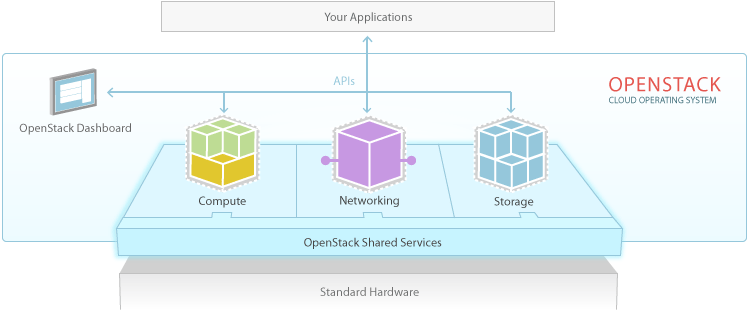
\includegraphics[width=\linewidth]{openstack-software-diagram}}
            \caption{OpenStack Software \cite{openstack_software}}
        \end{figure}
        
        
        OpenStack est à ce jour composé de 17 logiciels (modules) mais nous nous intéresserons à un seul : Nova.
        \begin{quote}
            \textit{«Nova dirige le cycle de vie des instances de calcul dans un environnement OpenStack. Les responsabilités de Nova englobent la création, l'ordonnancement et le démantèlement des machines virtuelles sur demande.» \cite{openstack_nova}}
        \end{quote}
        \bigbreak
        
        % ##############################################
        % On utilise que le commandes nova mais je pense qui y avait pas glance, ou neutron, on pourrait rien faire vu qu'on aurait pas d'OS, ni de réseau (enfin réseau optionnel)... non ?
        % D'ailleurs dans le 2.1 on met tous les composants essentiels d'openstack....
        Nova gère la communication avec la plate-forme de virtualisation (l'hyperviseur KVM plus spécifiquement) intégrée au noyau Linux, permettant l'instantiation de plusieurs machines virtuelles sur une même machine physique.
        Nova est suffisant pour créer un environnement de cloud. En effet il permet de créer un ensemble de machines virtuelles connectées au réseau publique de la machine hôte, d'y installer un système d'exploitation ainsi que des serveurs ssh par exemple pour pouvoir ensuite s'y connecter à distance et installer les applications qu'il souhaitent, et les exécuter.

    \section{Problématique et objectifs du projet}
        
        Ce projet a pour mission principale la prise en main d'un environnement de cloud de type IaaS à travers OpenStack. Pour cela, nous devons mettre en oeuvre un système d'automatisation de déploiement d'applications sur des machines virtuelles.\bigbreak
        
        Avec ces objectifs, nous avons défini les problématiques suivantes :
        \begin{itemize}
            \item Comment utilisé OpenStack pour créer des machines virtuelles ?
            \item Comment installer et démarrer des applications sur les machines virtuelles ?
            \item Comment automatiser le déploiement d'applications sur des machines virtuelles ?
        \end{itemize}
        \bigbreak

	\section{Organisation du projet}
	
    	Afin de mieux déterminer les tâches à effectuer, nous avons d'abord réalisé le diagramme de Gantt suivant :
    	
    	\begin{figure}[H]
            \centering{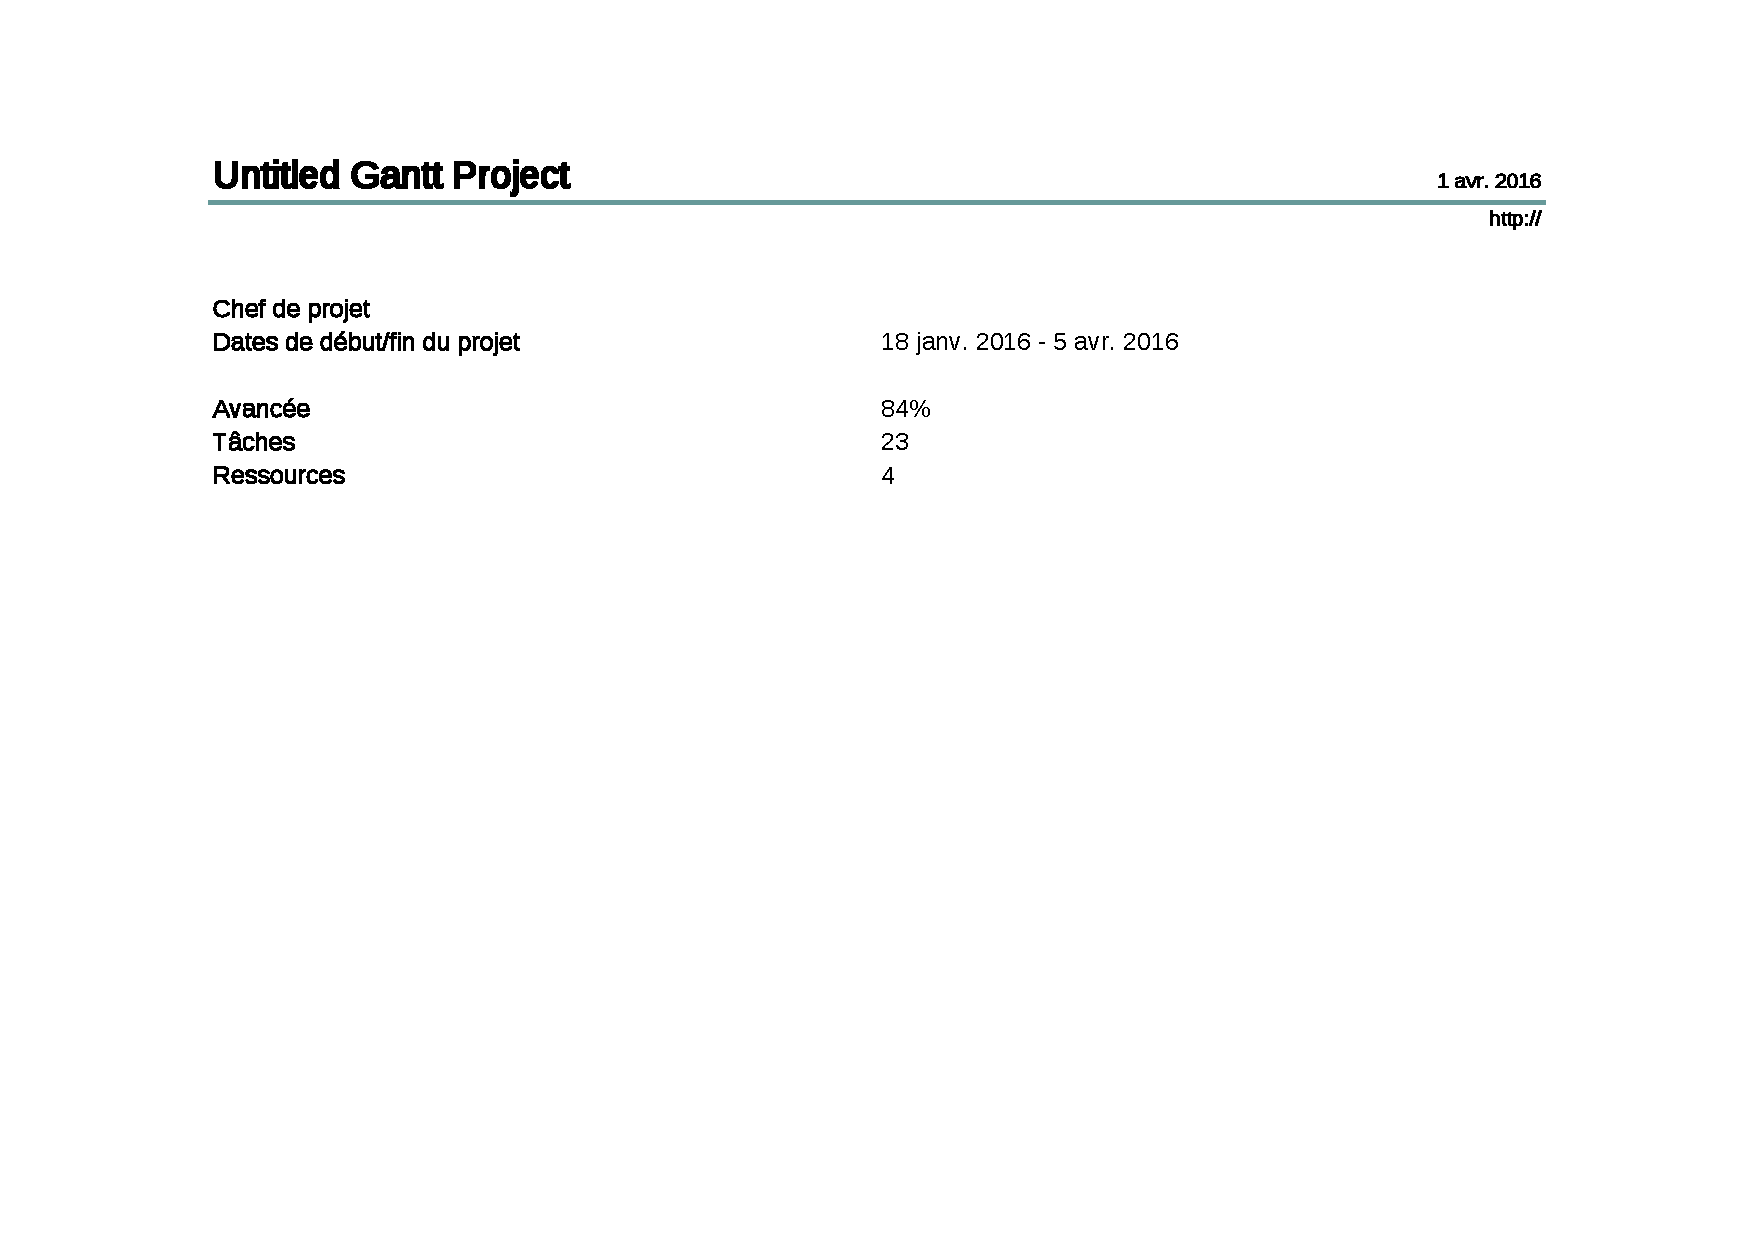
\includegraphics[width=\linewidth]{gantt}}
            \caption{Diagramme de Gantt}
        \end{figure}
    
        Tout au long du projet nous nous sommes réunis en moyenne deux après-midi par semaine pour travailler.
        Nous tenions aussi une réunion hebdomadaire avec notre tutrice de projet afin de l'informer de nos avancements et de lui demander des conseils.
        \bigbreak
    
        Dans la suite de ce rapport nous présenterons la prise en main de l'environnement OpenStack à travers nos premières expériences. Ensuite, nous développerons le travail effectué, notamment la conception de l'outil permettant le déploiement d'applications sur des machines virtuelles. Enfin, nous terminerons par un bilan de ce projet Cloud Computing à travers OpenStack.

    
% -------- CONTENU ----------
% ----------- 2 -------------
\newpage
\chapter{Prise en main d'OpenStack}

       OpenStack met à disposition deux solutions pour gérer son cloud. La première est une interface web appelée dashboard (en français tableau de bord), mis à disposition grâce au module Horizon. La deuxième est de passer par une interface de programmation applicative (souvent désignée par le terme API pour Application Programming Interface). C'est un ensemble normalisé de classes, de méthodes ou de fonctions qui sert de façade par laquelle un logiciel offre des services à d'autres logiciels. Afin d'atteindre nos objectifs, nous avons choisi d'utiliser l'API qui offre plus d'outils pour y parvenir.\bigbreak
       
      \textit{Vous trouverez en annexe x.x une capture d'écran de l'interface web Horizon.}
       
    \section{Installation d'OpenStack sur machines personnelles}

    %objectif initial : expliquer nos objectifs lors de l'installation d'OpenStack sur nos machines
    Dans l'objectif de déployer un environnement OpenStack nous avons choisi d'utiliser DevStack, un projet qui a pour but de rendre l'installation d'OpenStack accessible (avec peu de près-requis) avec un script permettant le téléchargement et la configuration de tous les composants essentiels à OpenStack.\cite{DevStack}\newline
    Nos objectifs étaient de déployer OpenStack sur nos machines de manière individuelle dans un premier temps puis de déployer OpenStack sur un réseau comprenant l'ensemble de nos machines par la suite.
    \bigbreak
    
    Il est conseillé d'utiliser DevStack sur des machines virtuelles car DevStack modifie la configuration réseau et la configuration des droits d'accès aux fichiers sur les machines hôtes.\newline
    % De plus, DevStack doit être redéployé à chaque démarrage de la machine hôte, ce qui constitue une contrainte supplémentaire.\newline
    %Face à celles-ci, notre tutrice nous a offert la possibilité d'utiliser d'un environnement OpenStack dédié à une plateforme distribuée existante nommée Grid'5000 et présentée dans la section suivante.
    Faisant face à plusieurs difficultés lors de l'installation et du déploiement de DevStack, notre tutrice nous a offert la possibilité d'utiliser d'un environnement OpenStack dédié à une plateforme distribuée existante nommée Grid'5000.


    \section{OpenStack sur une plateforme distribuée}

		\subsection{La plateforme Grid'5000}

La plate-forme Grid’5000 est une grille informatique, c’est-à-dire une infrastructure distribuée sur différents sites géographiques (Grenoble, Lyon, Toulouse, Bordeaux, Lille, Rennes, Reims, Nantes, Nancy, Luxembourg).
Elle a été créée par l'INRIA (Institut national de recherche en informatique et en automatique) afin de permettre des expériences à grande échelle dans le domaine informatique.
\cite{G5K}
\bigbreak

 Elle dispose de 1200 nœuds physiques. La totalité des nœuds représentent 2200processeurs, soit 8000 cœurs.  Les sites géographiques sont reliés par une fibre optique 10 Gbits/s faisant partie du réseau RENATER qui relie les différentes universités et centres de recherche français.
 
 \bigbreak

\begin{figure}[H]
        \centering{\includegraphics[scale=0.45]{grid5000}}
        \caption{Architecture de Grid'5000 \cite{archi_grid}} 
        \label{grid5000}
\end{figure}

Afin de se connecter à l’infrastructure G5K, il faut se connecter en SSH à acces.grid5000.fr, ce qui permet ensuite d’accéder aux différents sites sur lesquels il est possible d’effectuer des réservations de noeuds.
\bigbreak

		  \subsection{OpenStack sur Grid'5000 : XP5K-OpenStack}
		  
		     \begin{quote}  %%%%%%% à reprendre
                «XP5K est une bibliothèque légère écrite en Ruby permettant d'aider les utilisateurs de Grid'5000 à préparer leur expérimentations en faisant appel à l'interface de programmation Grid'5000 pour :
                \begin{itemize}
                \item Faire des réservations, voir le statut des réservations, supprimer une réservation...
                \item Créer des rôles (chaque nœud est dédié à un rôle, par exemple : contrôleur, unités de calcul), sans avoir à connaître le nom des nœuds qu'on utilise.
                \item Faire un ou plusieurs déploiement sur des nœuds spécifiés par une réservation ou un rôle.» \cite{XP5K}
                \end{itemize}
            \end{quote}
            
            \begin{quote}
		       «Puppet est un logiciel libre, écrit en Ruby, permettant la gestion de la configuration de serveurs esclaves. Il permet de gérer les déploiements système et applicatif.»
		       \cite{Puppet}
		    \end{quote}
		   
            XP5K-OpenStack est une interface de programmation conçue pour déployer OpenStack sur Grid'5000.
            XP5K-OpenStack utilise d'une part l'interface de programmation XP5K, permettant de manipuler les réservations et les nœuds sur Grid'5000, d'autre part l'outil de gestion de configuration Puppet configuré avec les modules Puppet-OpenStack qui, à partir d'un nœud maitre (le puppet master) permet le déploiement d'OpenStack sur un ensemble de nœuds de calcul (esclave).
            
		  \subsection{Déploiement et exécution d'applications sur XP5K-OpenStack}
Après avoir compris les bases et le fonctionnement sur XP5K-OpenStack, nous avons identifiés et listés les étapes nécessaires pour automatiser le déploiement des applications sur les machines virtuelles.\bigbreak

Une fois connecté sur Grid'5000 et XP5K-OpenStack importé sur le compte utilisateur, il faut l'éxécuter afin que celui ci déploie Openstack sur les noeuds réservés (durée de cette étape ~30 minutes).\bigbreak

Une fois fait, il faut créer et paramétrer les machines virtuelles. À la fin de cette étape, il ne manque qu'à importer les fichiers nécessaires à l'installation de l'application, ou directement l'exécutable sur les machines virtuelles. 
Enfin, la dernière étape est simplement d'exécuter la ou les applications via SSH.

    \section{Réfléxion sur l'automatisation}
    Avant de commencer le développement de l'outil permettant l'automatisation du déploiement d'applications sur des machines virtuelles, nous avons d'abord réfléchi sur les parties les plus importantes à automatiser. Par exemple, la création de la machine virtuelle avec les différents paramètres (nom, caractéristiques...) est un élément important de l'automatisation, tandis que l'importation des applications sur la plate-forme est un élément lié à l'environnement Grid'5000 et est donc moins important dans le cadre de ce projet.\bigbreak
    
    Une fois toutes ces réflexions faites, nous avons commencé à développer cet outil d'automatisation.



% -------- CONTENU ----------
% ----------- 3 -------------
\chapter{Un outil pour automatiser le déploiement et l'exécution d'applications sur OpenStack}
    
    Pour la réalisation d'un outil d'automatisation, nous avons choisi une implémentation basée sur des scripts écrits en Bash et en Ruby. Un script est un code interprété qui, à la manière d'un script au théâtre édicte une succession d'actions à réaliser.
    Dans le cadre de ce projet les scripts servent à exécuter et coordonner les commandes de Nova automatiquement.
    
    Afin de réaliser cette tâche, nous avons décidé de créer des "scripts"  Les scripts nous servent à exécuter et coordonner les commandes de Nova automatiquement. 
   
	%Paragraphe introductif : Quels sont les solutions techniques pour automatiser les tâches citées précedement afin de cacher les aspect techniques à l'utilisateur?
    
    Dans un premier temps ce chapitre présente l'aspect algorithmique, suivi de l'aspect technique des scripts développés.


    \section{Description générale}

    %algo : parser le fichier de configuration en un tableau
    %parcourir le tableau et creer les VM et installer les applications sur les VM
    La première étape du processus d'automatisation est la création d'un fichier de configuration structuré. Ce fichier contient des informations sur les machines virtuelles, tel que la puissance de calcul, le nombre et leur nom. Il contient aussi des informations sur les applications devant être installés comme le nom, le type (client, serveur, ...), le port si besoin. Dans un second temps, ce fichier est l'entrée d'un script (cf. p\pageref{construct} figure \ref{construct}) qui analyse ces informations et les redistribue au script de création de machines virtuelles (cf. p\pageref{vmsetup} figure \ref{vmsetup}) puis pour chacune d'entre elles appellent le script d'installation (cf. p\pageref{appsetup} figure \ref{appsetup}) avec les informations adaptées. \bigbreak
    
    %(cf. p\pageref{NoM} figure \ref{NoM})

    \section{Implémentation}
    
   \begin{itemize}
            
        \item % construct.rb
        \textbf{construct.rb} : analyse le fichier de configuration (config.json) et appelle les scripts de création de machine virtuelle (VMSetup.sh) et d'installation d'application (appSetup.sh).\newline
        \begin{algorithm}[H]
            \KwData{config.json}
            \SetAlgoLined
            \textbf{Begin}\newline
            décoder config.json\;
             \For{VM in VMs}{
                \For{1..nbClone}{
                    créer VM\;
                    \If{VM installée}{
                        \For{APP in APPs}{
                            installer APP\;
                        }
                    }
                }
             }
             \textbf{End}
            \caption{construct.rb}
        \end{algorithm}
        \bigbreak
    
        \item % VMSetup.sh
        \textbf{VMSetup.sh} : créé une machine virtelle.\newline
        \begin{Verbatim}[frame=single,fontsize=\normalsize,commandchars=\\\{\},label=Algorithme VMSetup]
Algorithme : VMSetup
Entrée :- tailleVM : taille de la machine virtuelle à créer. 
        - nomVM : nom de la machine virtuelle à créer.
Localisation : les commandes sont exécutées au niveau du controlleur, 
               là où OpenStack est installé et où l'on peut faire appel
               aux commandes Nova.

Debut :
    Vérification tailleVM valide.
    Vérification nomVM valide 
        ( nom n'étant pas déjà utilisé par une autre machine virtuelle ).
    Ajout de la clé de chiffrement dans la configuration Nova.
    Créer la machine virtuelle.
    Créer une IP publique.
    Récupérer adresse IP créée.
    Attribuer adresse IP à la machine virtuelle.
    Connection à la machine virtuelle.
    Mise à jour des briques logicielles de base.
    Fin de la connection.
Fin algorithme.
        \end{Verbatim}
    \bigbreak
    
        \begin{algorithm}[H]
          \SetAlgoLined
            \KwData{
                \begin{itemize}
                    \item tailleVM : taille de la machine virtuelle à créer.
                    \item nomVM : nom de la machine virtuelle à créer.
                \end{itemize}
                }
         
          Vérification tailleVM valide\;
          Vérification nomVM valide\;
          Ajout de la clé de chiffement dans la configuration Nova\;
          Créer la machine virtuelle\;
          Créer une IP publique\;
          Récupérer adresse IP créée\;
          Attribuer adresse IP à la machine virtuelle\;
          Connection à la machine virtuelle\;
          Mise à jour des briques logicielles de base.
          Fin de la connection.
     \caption{VMSetup.sh}
    \end{algorithm}
           
    \item %installation app
    \textbf{appSetup.sh} : installe et démarre une application.\newline
        
        \begin{algorithm}[H]
          \SetAlgoLined
            \KwData{
                \begin{itemize}
                \item nomVM : nom d'une machine virtuelle
                \item nomAPP : nom de l'application à installer
                \item typeApp : type d'application
                \item pathAPP : chemin vers le repertoire
                \item portAPP : port si application communicante
                \item serveurAPP : nom de la VM jouant le role de serveur
                \end{itemize}
                }
         \textbf{Begin}\newline
          Vérification de la validité des arguments\;
          Récupération de l'IP de la machine virtuelle ciblée par nomVM\;
          Copie des fichiers présents à pathApp vers la machine cible\;
          Connection à la machine cible\;
          Installation de l'application sur la machine cible\;
          \eIf{typeAPP == client}{
            On execute l'application en passant serveurAPP en paramètre\;
          }
          {
            On execute l'application sans argument\;
          }
          \textbf{End}
        
     \caption{AppSetup.sh}
    \end{algorithm}
    \bigbreak

    \end{itemize}
  

    \section{Vérification}

Pour les étapes où une vérification est nécessaire, Nova nous fournit deux commandes. La première: nova floating-ip-list, permet de voir la liste des IP créées.
  
  \begin{figure}[H]
            \centering{\includegraphics[width=\linewidth]{novafloatingip}}
            \caption{Affichage nova floating-ip-list}
  \end{figure}

La seconde: nova list, permet de voir les machines virtuelles créées ainsi que leurs caractéristiques, notamment si une IP a été liée à une machine.\bigbreak
  
  \begin{figure}[H]
            \centering{\includegraphics[width=\linewidth]{novalist}}
            \caption{Affichage nova list}
  \end{figure}


Pour vérifier l'exécution d'un programme, il y a principalement deux façons de faire, la plus simple étant de récupérer un résultat retourné ou un fichier de log. L'autre façon étant de se connecter à la machine virtuelle et de vérifier les processus actifs (par exemple: ps -ef | grep -o nom\_Du\_Prog).


    \section{Améliorations}
    %montrer comment on aurait pu faire un parseur avec Heat 
    %interface graphique ( automatiser la connection au point d'accès )
    %montrer comment on pourrait faire le déploiement des applications sur nos VM avec Puppet

    %Description pb JSON
    Pour configurer le déploiement d'applications avec notre outil, l'utilisateur doit manipuler un fichier de configuration au format JSON. Ce format ne permet pas facilement de décrire l'installation d'applications complexes, qui prendraient plusieurs paramètres, ou qui auraient par exemple un ensemble de machines virtuelles qui communiqueraient entre elles de manière plus complexe que le cas d'une application client serveur.
    \bigbreak
    
    %solution puppet
    Une solution pour configurer de manière plus simple le déploiement d'application serait d'utiliser Puppet qui permet de configurer et de déployer des applications complexes sur des machines virtuelles  grâce à des templates s'adaptant à la configuration de la machine.\newline
    Puppet reste peu accessible pour un utilisateur, mais offre la possibilité de déplacer les informations concernant la configuration des machines dans une base de donnée.\newline
    L'idée serait donc de créer une application graphique, facile d'utilisation pour l'utilisateur, qui modifiera une base de données dans laquelle Puppet irait chercher les informations pour configurer les noeuds.
    \bigbreak

    %screen
    Pour naviguer d'une machine virtuelle à l'autre, il est possible d'utiliser le programme Screen.
    \begin{quote}
        \textit{«Screen (GNU Screen) est un « multiplexeur de terminaux » permettant d'ouvrir plusieurs terminaux dans une même console, de passer de l'un à l'autre et de les récupérer plus tard.» \cite{Screen}}
    \end{quote}
    Screen permettant d'afficher plusieurs terminaux virtuels, notre programme pourrait utiliser Screen pour afficher les terminaux des différentes machines virtuelles sur une même fenêtre.\bigbreak
    \begin{figure}[H]
        \centering{}\includegraphics[width=\textwidth]{screen}
        \caption{Affichage de plusieurs terminaux virtuels sur une même fenêtre avec Screen \cite{imageScreen}} 
        \label{screen}
        \hspace{\linewidth}
    \end{figure}
    % python
    Les scripts ont d'abord été développés en Bash, mais nous avons ensuite trouvé une librairie Python qui permet de communiquer avec OpenStack directement. Il serait donc possible de n'utiliser qu'un seul langage, Python, pour tous nos scripts.


% ------- Conclusion --------
% ----------- 4 -------------
\newpage
\chapter{Conclusion}
    %Osef ce sont les objectifs ?
    L'objectif principal de ce projet était la prise en main d'un environnement de Cloud à travers OpenStack en mettant en oeuvre un système d'automatisation de déploiement d'applications sur des machines virtuelles.
    \bigbreak
    %Osef ça n'à rien à faire ici ~
    Après quelques difficultés liés à l'utilisation de DevStack, nous avons réussi à nous intégrer à la plateforme de Grid'5000. Petit à petit, nous avons réalisé des scripts réalisant des parties de notre objectif, pour arriver à la fin à un script global qui permet d'automatiser le déploiement de une ou plusieurs applications sur une ou plusieurs machines virtuelles.
    \bigbreak
    
    L'utilisation de Grid'5000 nous a permis d'acquérir d'importantes notions sur les infrastructures informatiques distribuées.
    \bigbreak
    
    Ce projet nous a aussi permis d'acquérir compétences et notions dans le domaine du Cloud Computing. %encore heureux
    
 
% --- BIBLIOGRAPHIE ---
\newpage

\printbibliography


% ---- ANNEXES ----
\newpage
\chapter*{Annexes}
    \begin{figure}[H]
        \centering{}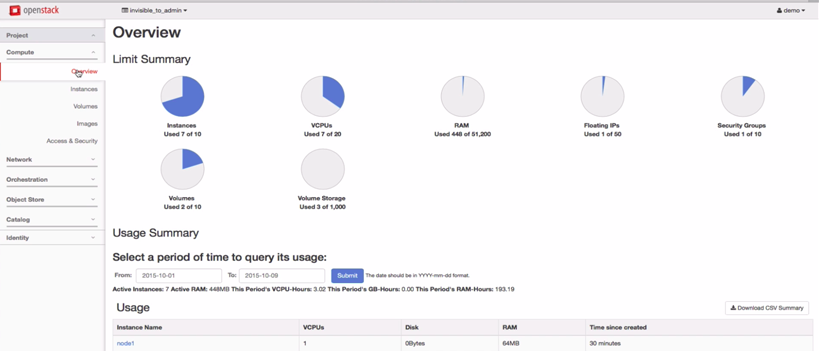
\includegraphics[width=\textwidth]{dash}
        \caption{Interface web Horizon (dashoard)}
        \label{dashboard}
    \end{figure}

%workpackage.
    \begin{figure}[H]
        \centering{}\includegraphics[width=\textwidth]{workpack}
        \caption{Liste des tâches de notre diagramme de gantt}
        \label{gantt}
    \end{figure}
    
    
    \begin{figure}[H]
        \centering{}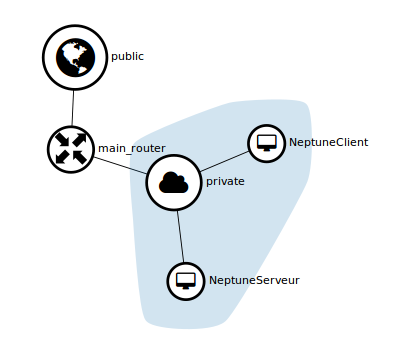
\includegraphics[width=\textwidth]{network-topo.png}
        \caption{Vue du cloud offerte par Horizon} 
        \label{cloudHorizon}
    \end{figure}
    
    
    
    \newpage
\begin{center}
        VM\_Setup.sh
    \end{center}
    \begin{verbatim}
#!/bin/bash

ERR_ARGS=-1

if [ $# -ne 2 ]; then
  echo "Usage: `basename $0` taille_VM nom_VM"
  exit $ERR_ARGS
fi

echo "- Vérification de la taille de la VM ($1)";
case $1 in
    xs|small|medium|large|xlarge)
        ;;
    *)
        echo "taille_VM: xs | small | medium | large | xlarge : $1";
        exit $ERR_ARGS;;
esac

mkdir -p logs/$2/
LOG="logs/$2/VMSetup.log"

# On récupère l'adresse du controller
ADR=`rake roles:show | grep 'controller' | grep -o -E '[^: ]*\.grid5000\.fr'`;
echo "# Controleur: $ADR" >> $LOG

KEYPAIR=`ssh root@$ADR 'source openstack-openrc.sh && nova keypair-list' | grep -o -E 'mainKey'`;
if [ -z $KEYPAIR ]; then
        echo "- Ajout de la Key Pair";
        cat ~/.ssh/id_rsa.pub | ssh root@$ADR "source openstack-openrc.sh && nova keypair-add --pub_key - mainKey"
fi

NOMSVMS=`ssh root@$ADR 'source openstack-openrc.sh && nova list' | cut -d '|' -f 3 | grep -o -E '([a-zA-Z0-9_]+)' | grep -v 'Name'`;

echo "- Vérification du nom de la VM ($2)";
if ! [[ "$2" =~ ^[a-zA-Z0-9_]+$ ]]; then
    echo "Le nom de la VM doit être alphanumerique (a-zA-Z0-9_)"
    exit $ERR_ARGS
fi
for NOMVM in $NOMSVMS; do
	if [ "$NOMVM" = "$2" ]; then
	    echo "Le nom de la VM $2 existe déjà, veuillez en choisir un autre"
	    exit $ERR_ARGS
	fi
done

echo "- Création de la VM...";
rake cmd cmd="
echo '# Execution du source openstack';
source openstack-openrc.sh;

VAR_RULE=\`nova secgroup-list-rules default | grep -o 10000\`;
if [ -z \"\$VAR_RULE\" ]; then
        echo '# Ajout des regles du parfeu'
        nova secgroup-add-rule default tcp 10000 10100 0.0.0.0/0;
        nova secgroup-add-rule default udp 10000 10100 0.0.0.0/0;
fi

echo '# Creation de la VM';
nova boot --flavor m1.$1 --image 'Debian Jessie 64-bit' --nic net-id=\$(neutron net-show -c id -f value private) --key_name mainKey $2

echo '# On attend que la VM soit disponible';
while [ \"\`nova list --name $2 | grep -o -E 'ACTIVE|ERROR'\`\" != 'ACTIVE' ]; do
    if [ \"\`nova list --name $2 | grep -o -E 'ACTIVE|ERROR'\`\" = 'ERROR' ]; then
        nova delete $2;
        nova boot --flavor m1.$1 --image 'Debian Jessie 64-bit' --nic net-id=\$(neutron net-show -c id -f value private) --key_name mainKey $2
    fi
    sleep 2;
done

echo '# Creation de l IP publique';
IP_PUB=\`nova floating-ip-create public | grep -o -E '(([0-9]{1,3}\.){3}[0-9]{1,3})'\`;
echo \"# Ajout de l IP publique (\$IP_PUB) a la VM\";
nova add-floating-ip $2 \$IP_PUB;
" host=controller >> $LOG

echo "- VM créée";

# Connexion au controleur pour récupèrer l'IP de la VM
IP=`ssh root@$ADR "source openstack-openrc.sh && nova list --name $2" | grep -o -E '(10\.([0-9]{1,3}\.){2}[0-9]{1,3})'`;

echo "- En attente de connexion ssh disponible ($IP)";
while ! ssh -q debian@$IP 'exit'; do
    sleep 2;
done

echo "- Mise à jour de la VM...";
ssh -q debian@$IP "sudo apt-get -y update; sudo apt-get -y install gcc make;" >> $LOG;
echo "- Mise à jour réussie";

exit 0
    \end{verbatim}
    
    
    
    
    \newpage
    \begin{center}
        APP\_Setup.sh
    \end{center}
    \begin{verbatim}
#!/bin/bash

ERR_ARGS=-1

if [ $# -ne 5 ] && [ $# -ne 6 ]; then
    echo "Usage: `basename $0` nom_VM nom_APP type_APP path_APP port_APP [type_APP=client=>serveur_APP]"
    exit $ERR_ARGS
fi

echo "- Vérification du type de l'application et des parametres";
case $3 in
    client)
    if [ $# -ne 6 ]; then
        echo "Usage: `basename $0` nom_VM nom_APP type_APP path_APP port_APP serveur_APP"
        exit $ERR_ARGS
    fi
    ;;
    normal)
	;;
    serveur)
    echo "- Vérification du port de l'application";
    if [ $5 -lt 10000 ] && [ $5 -gt 10100 ]; then
        echo "port_APP: 10000 à 10100 : $5"
        exit $ERR_ARGS
    fi	
    ;;
    *)
    echo "type_APP: client | serveur | normal : $3"
    exit $ERR_ARGS;;
esac

mkdir -p logs/$1/
LOG="logs/$1/appSetup.log"

# On récupère l'adresse du controller
ADR=`rake roles:show | grep 'controller' | grep -o -E '[^: ]*\.grid5000\.fr'`;

# On se connecte au controleur pour récupérer l'IP de la VM
IP=`ssh root@$ADR "source openstack-openrc.sh && nova list --name $1" | cut -d '|' -f 7 | grep -o -E '(10\.([0-9]{1,3}\.){2}[0-9]{1,3})'`;

if [ "$3" = "client" ]; then
    # On se connecte au controleur pour récupérer l'IP de la VM serveur
    IPServeur=`ssh root@$ADR "source openstack-openrc.sh && nova list --name $6" | cut -d '|' -f 7 | grep -o -E '(10\.([0-9]{1,3}\.){2}[0-9]{1,3})'`;
    echo "IP VM serveur : $6:$IPServeur"
    if [ -z "$IPServeur" ]; then
        echo "L'IP de la VM serveur est introuvable"
        exit $ERR_ARGS
    fi
fi

echo "- Copie de l'application ($2) sur la VM"
scp -q -p -r $4 debian@$IP: >> $LOG

echo "- Démarrage de l'application"
if [ "$3" = "client" ]; then
    ssh -q debian@$IP "cd $2; make $3; ls -l; ./$3 $IPServeur $5" >> $LOG &
else
 	ssh -q debian@$IP "cd $2; make $3; ls -l; ./$3 $5" >> $LOG &
fi

exit 0
    \end{verbatim}
\end{document}


% --------------------------- INSTALLATION LATEX ----------------------
%sudo apt-get install texlive
%sudo apt-get install texlive-lang-french
%sudo apt-get install texlive-latex-extra
% Compile Time : pdflatex Rapport.tex
% Pensez à virer les .log, .aux, .out ET .pdf avant de push !
